\documentclass{llncs}
% Grundgröße 12pt, zweiseitig
% Standardpakete
% richtiges encoding fuer verschiedene compiler
\usepackage{iftex}
\ifPDFTeX
   \usepackage[utf8]{inputenc}
   \usepackage[T1]{fontenc}
   \usepackage{lmodern}
\else
   \ifXeTeX
     \usepackage{fontspec}
   \else 
     \usepackage{luatextra}
   \fi
   \defaultfontfeatures{Ligatures=TeX}
\fi
% deutsche Silbentrennung
\usepackage[english]{babel}
\usepackage{amsmath}
\usepackage{cite}
\usepackage{float}
\usepackage{subfig}

% Grafiken einbinden
\usepackage{graphicx}
\graphicspath{{figures/}}

\usepackage{hyperref}
% tiefe des Inhaltsverzeichnisses
\setcounter{tocdepth}{2}


\begin{document}

\title{Project proposal: Comparative exploration of Abalone game-playing agents}
\author{Ture Claußen, 202132027, \email{ture.claussen@stud.hs-hannover.de}}
\authorrunning{T. Claußen}
\institute{Dept. of Software and Computer Engineering, Ajou University}

% jetzt gehts los
{\def\addcontentsline#1#2#3{}\maketitle} % Wird gebraucht, damit der Title nicht im Inhaltsverzeichnis steht

\begin{abstract}
  Games provide the perfect environment for artificial agents to navigate in. Especially for the
  \keywords{AI \and Alpha-beta \and Q-Learning \and Abalone \and Intelligent Agents}
\end{abstract}

\section{Introduction}

Abalone is a fairly new game, that was devised in 1987 by Michel Lalet and Laurent Lévi. Nevertheless, with more than four million global sales it could establish itself as a classic game \cite{noauthor_abalone_2020}. Ablalone is a two-player game consisting of a hexagonal board with 61 fields and 14 marbles for black and white respectively. The abstract nature of the game requires the player to plan ahead and find the right strategy in the plethora of moves. The goal is to create an agent that is up to par with a human player and moreover, has realistic computational requirements and reacts quickly.

In search of the optimal move it is not possible to expand all of the possible paths the game could take, even for modern computers. Hence, more sophisticated approaches for navigating the state space and evaluating good paths are needed. On the other hand, the game does not have piece-specific rules or large distance moves which reduces the need for a very domain specific knowledge about the game like e.g. for chess to find sensible heuristics.

Overall, this complexity makes the game a good project for the design of a game playing-agent, as it is meant to be an opportunity to apply the fundamental principles and algorithms learned, as opposed to being distracted by the engineering aspects. This matches my personal background on the subject matter, as I have no prior (formal) exposure to the design of artificial intelligence. Over the course of my current study of applied computer science I gained versatile proficiency in programming and the handling of data which will help implementing the algorithms efficiently and provide the epirical foundation for the paper.

\subsection{Survey}

Considering the existing landscape of papers, there is unquestionably a wide array of papers exploring the application of minimax and alpha-beta pruning on the game of Abalone. Some of the most prominent include:

\begin{enumerate}
  \item "Algorithmic fun-abalone" (2002) \cite{aichholzer_algorithmic_2002}
  \item "A Simple Intelligent Agent for Playing Abalone Game: ABLA" (2004)\cite{ozcan_simple_2004}
  \item "Constructing an abalone game-playing agent" (2005)  \cite{lemmens_constructing_2005}
  \item "Implementing a computer player for abalone using alpha-beta and monte-carlo search" (2009)\cite{chorus_implementing_2009}
\end{enumerate}

\subsection{Rules}

The goal of the game is to push six of the opponent's marbles off the playing field. The game's starting position is depicted in figure \ref{basics} (a). One, two, or three adjacent marbles (of the player's own color) may be moved in any of the six possible directions during a player's turn. We differentiate between broadside or "side-step" moves and "in-line" moves, depending on how the chain of marbles moves relative to its direction, which is shown in figure \ref{basics} (b) and (c).

\begin{figure}[!h]
  \centering
  \subfloat[Starting position]{
    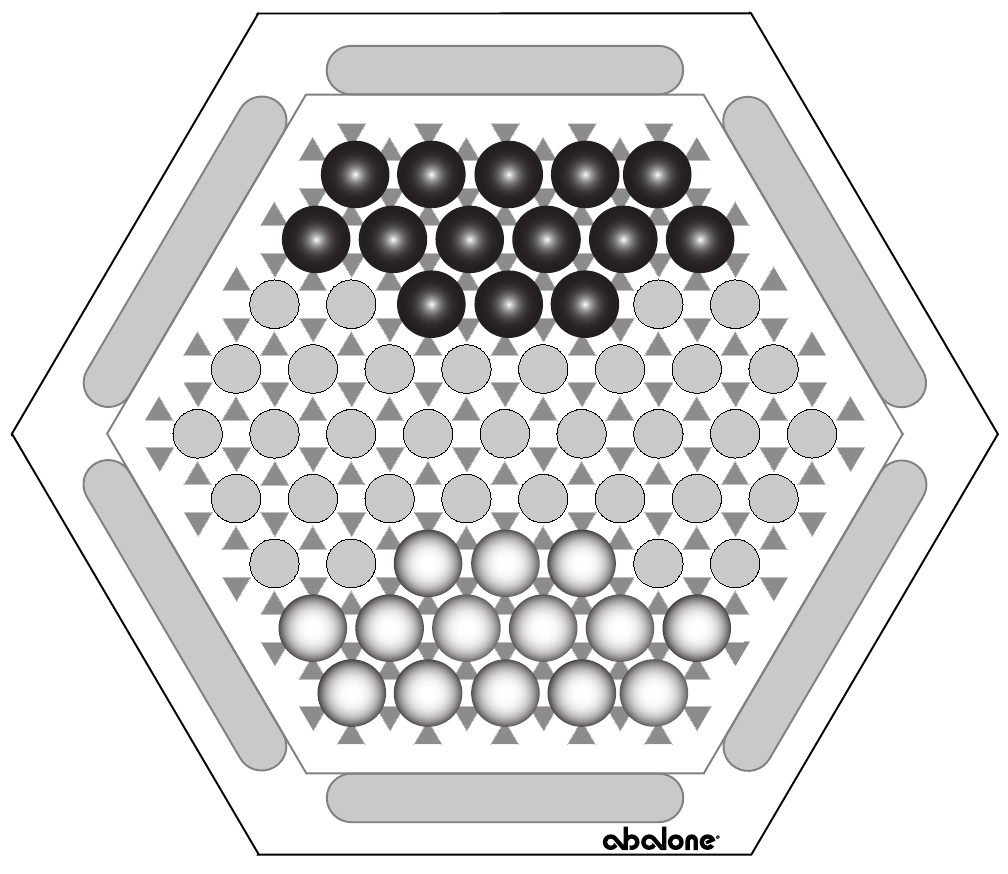
\includegraphics[width=3cm, keepaspectratio]{rules_starting_position.png}
  }
  \hfill
  \subfloat["In-line" moves]{
    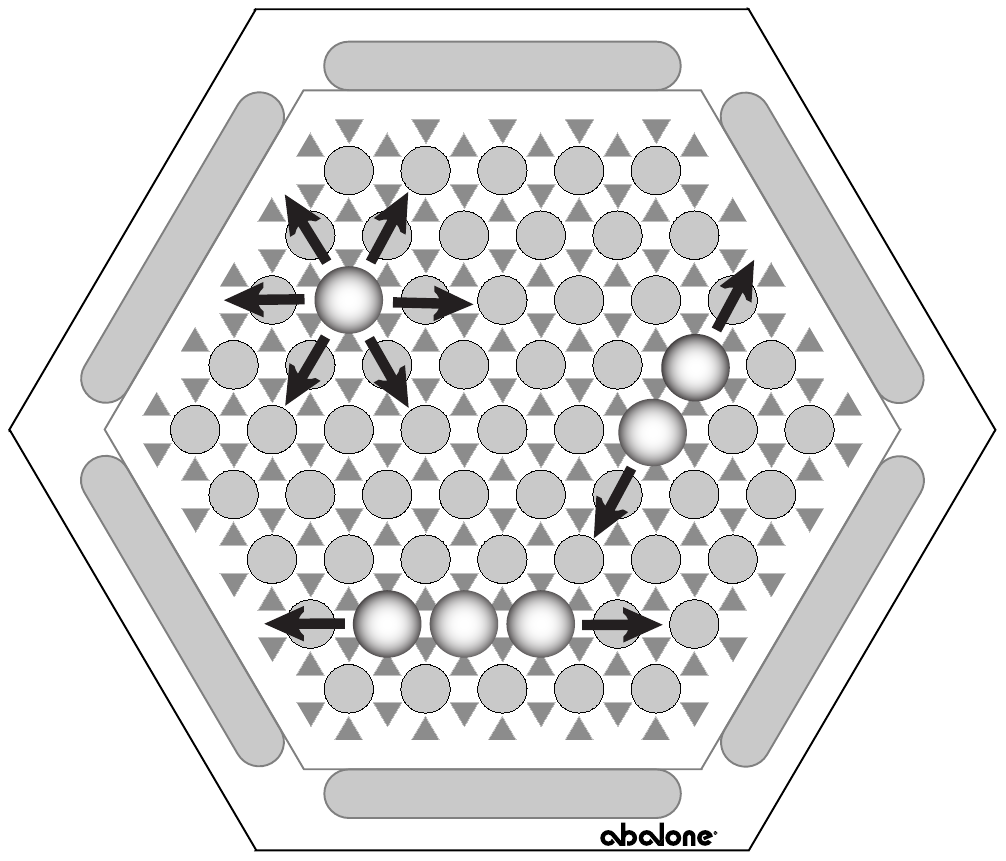
\includegraphics[width=3cm, keepaspectratio]{rules_inline_move.png}
  }
  \hfill
  \subfloat["Side-step" moves]{
    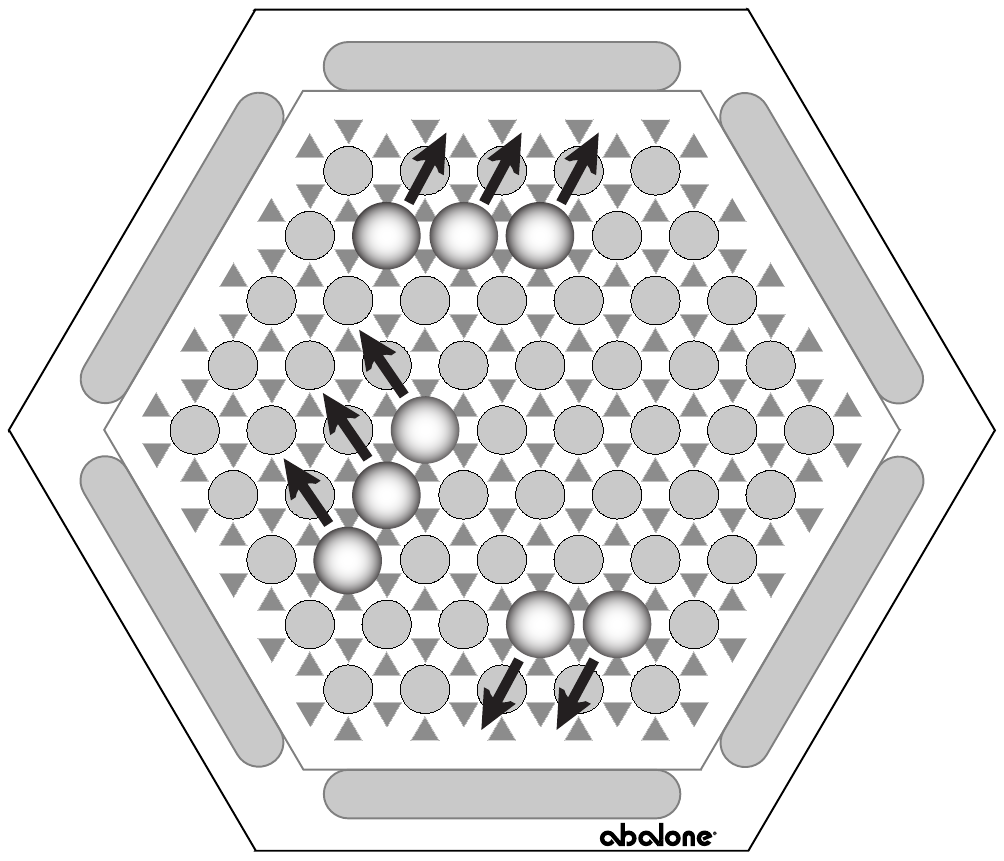
\includegraphics[width=3cm, keepaspectratio]{rules_side_step_move.png}
  }
  \caption{Basic moves \cite{abalone_sa_abalone_nodate}}
  \label{basics}
\end{figure}

\begin{figure}[!h]
  \centering
  \subfloat["2-push-1" sumito]{
    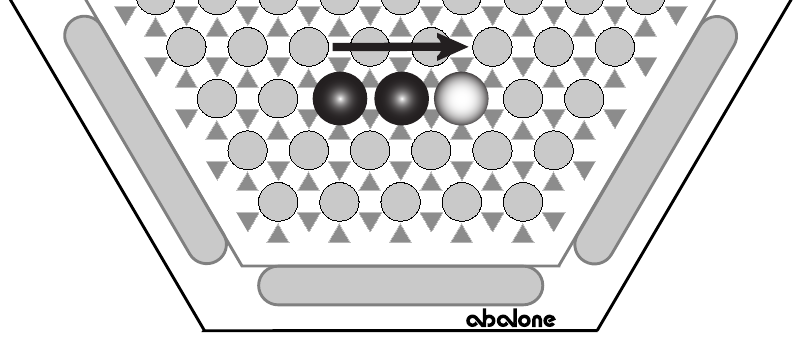
\includegraphics[width=3cm, keepaspectratio]{rules_2-push-1_sumito.png}
  }
  \hfill
  \subfloat["3-push-1" sumito]{
    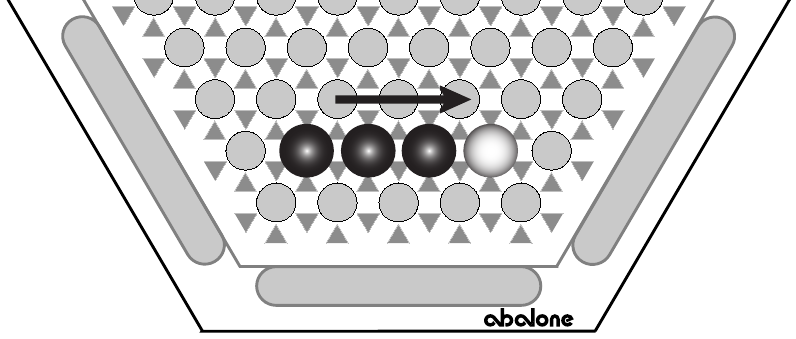
\includegraphics[width=3cm, keepaspectratio]{rules_3-push-1_sumito.png}
  }
  \hfill
  \subfloat["3-push-2" sumito]{
    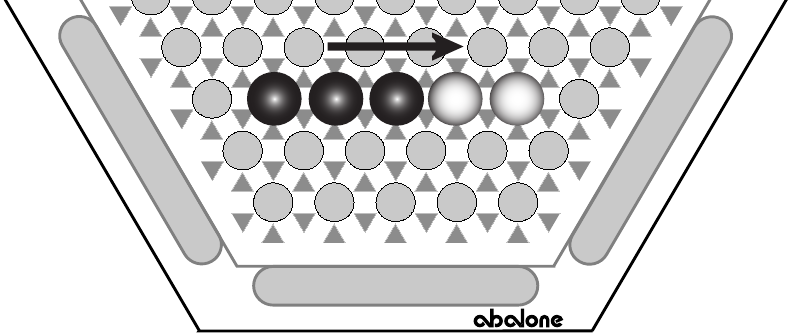
\includegraphics[width=3cm, keepaspectratio]{rules_3-push-2_sumito.png}
  }
  \caption{Sumito positions allow pushing the opponent's marbles \cite{abalone_sa_abalone_nodate}}
  \label{sumito}
\end{figure}

\subsection{Complexity}

\paragraph{State space complexity}

$$
  \sum_{k=8}^{14}\sum_{m=9}^{14}\frac{61!}{k!(61-k)!}\times\frac{(61-k)!}{m!((61-k)-m)!}
$$

\paragraph{Game tree complexity}

\paragraph{Comparative complexity}

\paragraph{Existing approaches}

\section{Project details}

\subsection{Agent design}

Based on the PEAS framework we can analyze the task environment for the agent. \cite[p.107]{russell_artificial_2021}

\begin{description}
  \item[Performance measure] Win/loss, number of moves, time to deliberate
  \item[Environment] Digital playing board
  \item[Actuators] Move marbles, display text to CLI
  \item[Sensors] Position of marbles
\end{description}

\subsection{Algorithm comparision}

\paragraph{Alpha-beta pruning}

\paragraph{Monte Carlo Tree Search}

\paragraph{Q-Learning}

\subsection{Timeline}

\section{Conclusion}

% Literatur
\bibliographystyle{splncs04.bst}
\bibliography{ref.bib}
\end{document}